\documentclass[10pt,letterpaper]{article} 
\usepackage{tikz}
\usepackage{tools}
\usepackage{enumitem}
%\usepackage{graphicx}‎‎
%\usefonttheme{serif}‎
%\usepackage{ptext}‎
%\usepackage{xepersian}
%\settextfont{B Nazanin}
\usepackage{lipsum}
\setlength{\parindent}{0pt}
\newcommand{\pf}{$\blacksquare$}

\newcommand{\bns}{\textit{broadcast-and-select}  architecture}
\newcommand{\Bns}{\textit{Broadcast-and-select} architecture}

\newcommand{\rns}{\textit{route-and-select} architecture}
\newcommand{\Rns}{\textit{Route-and-select} architecture}

\newcounter{QuestionNumber}
\setcounter{QuestionNumber}{1}

\newcommand{\Q}{
\textbf{Question \theQuestionNumber)}
\stepcounter{QuestionNumber}
}

\newcommand{\EX}{\Bbb E}
\newcommand{\nl}{\newline\newline}
\begin{document}
\Large
\begin{center}
In the name of beauty

The 4th problem set solution of Optical Networks course
\hl
\end{center}
\Q

\begin{enumerate} [label=\alph*-]
\item
The RRC filter bandwidth is given by $(1+\beta)R_s$ where $\beta$ is the roll-off factor and $R_s$ is symbol rate. A simple substitution yields 36Gbaud and 18Gbaud for its double-sided and single-sided bandwidth, respectively.
\item
To sample a RRC filter with bandwidth 36G, we need to sample the continuous signal once every 1/36 nsec ($f_{\text{sampling}}$=36G) to avoid aliasing.
\item
Denote the unencoded bit stream by $b_n$. When passing through the \textbf{bit-to-symbol converter}, the stream turns into $s_n$ which is a sequence of symbols, e.g. each of which chosen from the alphabet $\{-1-j,-1+j,1-j,1+j\}$ for PM-QPSK. Hence, the output becomes
$$
\sum_{n=-\infty}^{\infty} b_n\delta(t-nT_s),
$$
which has an inphase component of 
$$
\sum_{n=-\infty}^{\infty} \Re\{b_n\}\delta(t-nT_s)
$$
and a quadrature component of 
$$
\sum_{n=-\infty}^{\infty} \Im\{b_n\}\delta(t-nT_s).
$$
The operators $\Re$ and $\Im$ denote the real and imaginary parts of a complex variable, respectively.

The upsampler is a unit-gain, linear system block for sampling conversion and can be ignored since the discussion is fully taken place in analog regime. This leads to
%$$
%S(t)=\sum_{n=-\infty}^{\infty} b_n\delta(t-nT_s)
%$$
%Let's see what the Tx. output is. $S(t)$ passes through the \textbf{RRC pulse shaping block} which, as the name suggests, turns the ``impulse shape'' of the symbols in analog to ``RRC shape''. So far, the signal is constructed in baseband and is given by
$$
S(t)=\sum_{n=-\infty}^{\infty} \Re\{b_n\}s_\text{RRC}(t-nT_s),
$$
where $s_\text{RRC}(t)$ is the RRC pulse shape in time domain. The signal $S(t)$ is once multiplied in $\cos$ carrier and once in $\sin$ carrier to give the Tx. midband output signal as
\qn{
x(t)&=2\sum_{n=-\infty}^{\infty} \Re\{b_n\}s_\text{RRC}(t-nT_s)\cos 2\pi f_ct
\\&-
2\sum_{n=-\infty}^{\infty} \Im\{b_n\}s_\text{RRC}(t-nT_s)\sin 2\pi f_ct
}{}which is directly input to Rx. block diagram based on back-to-back connection. The upper and lower branch signals after multiplying in $\cos$ and $-\sin$ become

\qn{
x(t)\cos 2\pi f_c t&=
2\sum_{n=-\infty}^{\infty} \Re\{b_n\}s_\text{RRC}(t-nT_s)\cos^2 2\pi f_ct
\\&-
2\sum_{n=-\infty}^{\infty} \Im\{b_n\}s_\text{RRC}(t-nT_s)\sin 2\pi f_ct\cos 2\pi f_ct
\\&=
\sum_{n=-\infty}^{\infty} \Re\{b_n\}s_\text{RRC}(t-nT_s)(\cos 4\pi f_ct-1)
\\&-
\sum_{n=-\infty}^{\infty} \Im\{b_n\}s_\text{RRC}(t-nT_s)\sin 4\pi f_ct
}
and
\qn{
x(t)\sin 2\pi f_c t&=
\sum_{n=-\infty}^{\infty} \Re\{b_n\}s_\text{RRC}(t-nT_s)\sin 4\pi f_ct
\\&-
\sum_{n=-\infty}^{\infty} \Im\{b_n\}s_\text{RRC}(t-nT_s)(1-\cos 4\pi f_ct)
.
}
The $\cos 4\pi f_ct$ and $\sin 4\pi f_ct$ are modulated by a baseband signal to midband frequency $2f_c$ and are not passed through the ideal low-pass filter. Hence the output of the filter is
\qn{
\text{Output of the LPF}=\sum_{n=-\infty}^{\infty} \Re\{b_n\}s_\text{RRC}(t-nT_s),
}
which turns into 
$$
Y(t)=\sum_{n=-\infty}^{\infty} \Re\{b_n\}s_\text{RC}(t-nT_s)
$$
after passing through the RRC matched filter (RRC pulse shape) block since
$$
s_\text{RRC}(t)*s_\text{RRC}(t)=s_\text{RC}(t).
$$
\item
The above reasoning makes it clear as to why LPF is needed. We need LPF to extract the baseband signal out from a total received, midband signal since our pure information lays there.
\item
The output process of a LTI system with impulse response of $H(f)$ and a WSS input process with a PSD of $G(f)$ is WSS with a PSD of $G(f)|H(f)|^2$. Since $|H(f)|=1$, the PSD of input and output processes are equal and both of them are Gaussian processes with the same variance.
\end{enumerate}

\Q

\begin{enumerate}[label=\alph*-]
\item
We have 4 inner points of power $1^2+1^2=2$, 8 points with power $1^2+3^2=10$ and 4 corner points with equal power $3^2+3^2=18$, all of which equally likely. Hence the average power is 
$$
{1\over 16}(4\times 2+8\times 10+4\times 18)=10
$$
\item
The desired average power is assumed 6.6, which is
$$
2P_1+10P_2+10P_3+18P_4=6.6
$$
or equivalently
$$
2P_1+78P_4=6.6
$$
also
$$
P_1+P_2+P_3+P_4=1\implies P_1+7P_4=1
$$
with the following solution
\qn{
&P_1=0.496
\\&P_2=0.216
\\&P_3=0.216
\\&P_4=0.072
}
\item
$$
H\approx3.04\text{ bits}
$$
\end{enumerate}

\Q

\begin{enumerate}[label=\alph*-]
\item
\qn{
P_{\text{correct},1+1j}&=\Pr\{0<n_1+1<2,0<n_2+1<2\}
\\&=\Pr\{-1<n_1<1,-1<n_2<1\}
\\&=\Pr\{-1<n_1<1\}\cdot\Pr\{-1<n_2<1\}
\\&=(Q(\frac{-1}{\sigma})-Q(\frac{1}{\sigma}))^2
\\&=[1-2Q(\frac{1}{\sigma})]^2
\\&=\left[1-2Q\left(\sqrt{\frac{\text{SNR}}{5}}\right)\right]^2
,
}
\qn{
P_{\text{correct},1+3j}&=\Pr\{0<n_1+1<2,2<n_2+3<\infty\}
\\&=\Pr\{-1<n_1<1,-1<n_2\}
\\&=\Pr\{-1<n_1<1\}\cdot\Pr\{-1<n_2\}
\\&=(Q(\frac{-1}{\sigma})-Q(\frac{1}{\sigma}))\cdot Q(\frac{-1}{\sigma})
\\&=\left[1-2Q\left(\sqrt{\frac{\text{SNR}}{5}}\right)\right]\cdot \left[1-Q\left(\sqrt{\frac{\text{SNR}}{5}}\right)\right],
}
\qn{
P_{\text{correct},3+3j}&=\Pr\{2<n_1+3<\infty,2<n_2+3<\infty\}
\\&=\Pr\{-1<n_1,-1<n_2\}
\\&=\Pr\{-1<n_1\}\cdot\Pr\{-1<n_2\}
\\&=Q^2(\frac{-1}{\sigma})
\\&=\left[1-Q\left(\sqrt{\frac{\text{SNR}}{5}}\right)\right]^2
,
}
hence
\qn{
&P_{\text{error},3+3j}=1-P_{\text{correct},3+3j}
\\&P_{\text{error},1+3j}=1-P_{\text{correct},1+3j}
\\&P_{\text{error},1+1j}=1-P_{\text{correct},1+1j}
.
}
\begin{figure}[h]
\centering
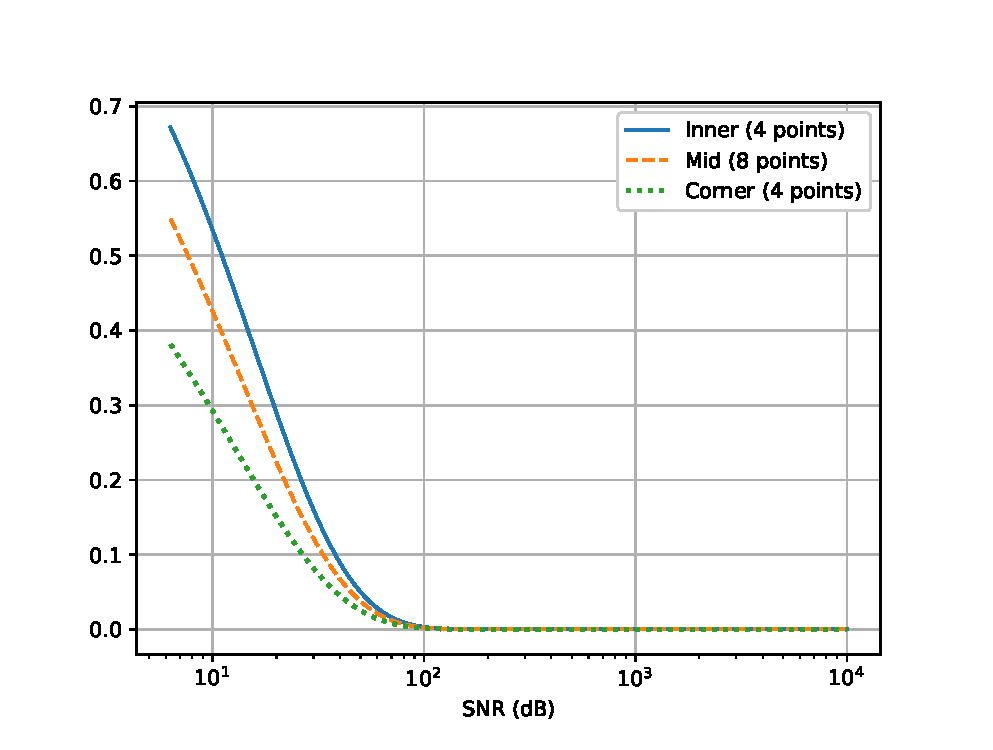
\includegraphics[width=120mm]{p_error_cond}
\caption{Conditional probabilities of symbols}
\end{figure}
\item
\begin{figure}[h]
\centering
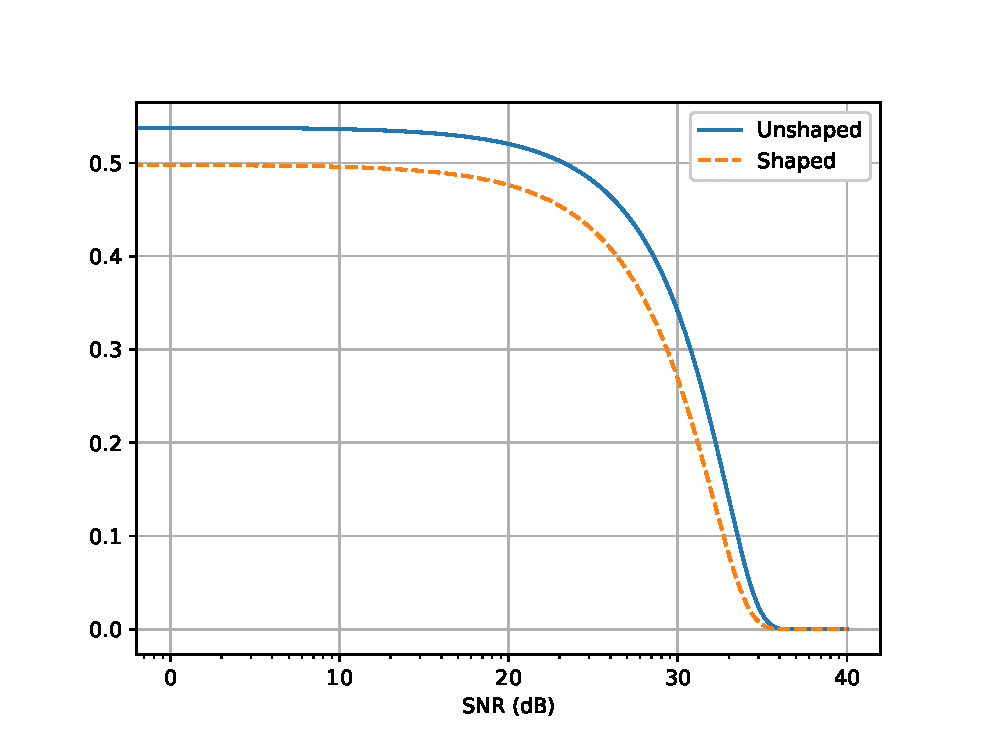
\includegraphics[width=120mm]{p_error_total}
\caption{Conditional probabilities of symbols}
\end{figure}
\end{enumerate}

\Q

\begin{enumerate}[label=\alph*-]
\item
Each 4 bits of an input stream are mapped to a symbol in 16QAM, leading to a bit rate of 96 Gbps.
\item
Since the channel encoder adds redundant bits to the input bit stream, each 3 input bits are mapped to 4 bits, thereby yielding a total bit rate of
$$
96\times {4\over 3} Gbps=128 Gbps
$$
\item
$$
96\times {6\over 5} Gbps=115.2 Gbps
$$
which is less than that in part b- since the redundancy is decreased.
\item
For unshaped 8QAM and 32QAM, the bit-to-symbol conversion ratio is 3 and 5, respectively, hence
\qn{
&\text{8QAM uncoded bit rate}=24\times 3=72Gbps
\\&
\text{32QAM uncoded bit rate}=24\times 5=120Gbps
}
similarly
\qn{
&\text{8QAM encoded bit rate}=24\times 3=86.4Gbps
\\&
\text{32QAM encoded bit rate}=24\times 5=144Gbps
}
\item
The bit-to-symbol ratio can be calculated from 
$$
H=-\sum_{i=1}^{16} \hat P_i\log_2 \hat P_i
$$
which with the probabilisitic shaping parameters calculated in question 2, gives 
$$
H=3.04 \text{ bits}
$$
\item
The bit rate is correspondingly equal to $24 G\times 3.04=72.96 \text{ Gbps}$, which when encoded, increases by ${6\over 5}$ to $87.55\text{ Gbps}$, though less than $115.2 Gbps$ since the number of bits per symbol is reduced.
\end{enumerate}

\Q

a and b. The ASE power spectral density is
\qn{
\sigma^2_\text{ASE,PSD}={1\over 2}N_\text{Span}h\nu_\text{opt} GF=16.06\mu\text{W/Gbaud}
}
hence the ASE noise variance becomes
\qn{
\sigma^2_\text{ASE}&=R_\text{Receiver}\sigma^2_\text{ASE,PSD}\\&=
(1+\beta)R_s\sigma^2_\text{ASE,PSD}\\&=0.462 \text{mW}\equiv -3.35 \text{dBm}
}{}
and the SNR is calculated as
$$
\text{SNR (dB)}=\text{Power (dBm)}-\sigma^2_{ASE}\text{ (dBm)}=12.75 \text{dB}
$$
c. A LDPC code with parameters (16193,9713) is needed to obtain a probability of error as $\sim 2\times 10^{-3}$. With such probability of error, a RS code with parameters (294,244) can reduce the probability of error by an astounding factor to $10^{-10}$.

d. That probabilistic shaping reduces the launch power by 32\% and hence the SNR; therefore
$$
\text{SNR}_{\text{Shaped}}=11.08\text{ dB}
$$
with an approximate probability of error of $\sim 5\times 10^{-3}$. Similarly, the LDPC and RS code parameters are (16195,12595) and (294,244) and the reduced probability of error is $\sim 10^{-6}$, respectively.
\end{document}